\documentclass[a4paper,14pt]{extarticle}
\usepackage{../../tex-shared/report-layout}

\renewcommand{\mylabnumber}{9}
\renewcommand{\mylabtitle}{Исследование возможностей хранения данных на стороне
сервера. Работа с файлами. Работа с реляционными СУБД.}
\renewcommand{\mysubject}{Веб-технологии}
\renewcommand{\mylecturer}{Овчинников А.Л.}

\begin{document}
\begin{titlepage}
    
    \thispagestyle{empty}
    
    \begin{center}
        
        Министерство науки и Высшего образования Российской Федерации \\
        Севастопольский государственный университет \\
        Кафедра ИС
        
        \vfill

        Отчет \\
        по лабораторной работе №\mylabnumber \\
        \enquote{\mylabtitle} \\
        по дисциплине \\
        \enquote{\MakeTextUppercase{\mysubject}}

    \end{center}

    \vspace{1cm}

    \noindent\hspace{7.5cm} Выполнил студент группы ИС/б-17-2-о \\
    \null\hspace{7.5cm} Горбенко К. Н. \\
    \null\hspace{7.5cm} Проверил \\
    \null\hspace{7.5cm} \mylecturer

    \vfill

    \begin{center}
        Севастополь \\
        \the\year{}
    \end{center}

\end{titlepage}

\section{Цель работы}
Изучить возможности хранения данных на стороне сервера: работу c файлами и СУБД
MySQL из PHP, приобрести практические навыки организации хранения данных на
стороне сервера в файлах, в базах данных MySQL, а также овладение навыками
постраничного вывода данных.

\section{Задание на работу}
\begin{enumerate}
    \item Разработать базовый класс BaseActiveRecord для работы с базой данных,
          который реализует паттерн ActiveRecord (данный класс разместить в
          папке \slash my\_site\slash app\slash core).
    \item Для всех моделей, которые будут использоваться при выполнении данной
          лабораторной работы, создать классы, наследующие BaseActiveRecord. Для
          каждого из классов определить все поля и названия таблиц.
    \item Создать новую страницу "Гостевая книга". Страница должна содержать
          форму ввода (Фамилия, Имя, Отчество, E –mail, Текст отзыва), а также таблицу
          сообщений, оставленных пользователями.
    \item Реализовать страницу "Загрузка сообщений гостевой книги", содержащую
          форму загрузки подготовленного заранее файла messages.inc на сервер.
    \item Реализовать на странице "Тест по дисциплине" сохранение ответов
          пользователей и правильности ответов в разработанную таблицу базы данных
          MySQL, с возможностью просмотра сохраненных данных.
    \item Разработать страницу «Редактор Блога», позволяющую добавлять записи
          Блога. Страница должна содержать форму добавления записи Блога и список
          выдаваемых постранично записей отсортированных в порядке убывания даты.
    \item Разработать страницу \enquote{Мой Блог}, содержащую упорядоченные в порядке
          убывания даты добавления, выдаваемые постранично данные.
    \item Реализовать возможность добавления записей на страницу \enquote{Мой Блог} из
          файла формата CSV.
\end{enumerate}
\pagebreak

\section{Ход работы}
\subsection{Разработка класса BaseActiveRecord}
\begin{lstlisting}
abstract class BaseActiveRecord {
    protected static $pdo;
    private static $tablename;
    private static $className;
    private static $dbfields = array();

    protected $id;

    public function __construct() {
        static::setupConnection();
    }

    private static function setupConnection() {
        static::$pdo = PortfolioPdo::getInstance();
    }

    public static function find($id) {
        static::setupConnection();

        $sql = "SELECT * FROM " . static::$tablename . " WHERE id=$id";
        $stmt = static::$pdo->prepare($sql);
        $stmt->setFetchMode(PDO::FETCH_CLASS, static::$className);
        $stmt->execute();
        $result = $stmt->fetch();

        if (!$result) {
            throw new Exception("Entity " . static::$className . " was not found.");
        }

        return $result;
    }

    public static function findAll() {
        static::setupConnection();

        $sql = "SELECT * FROM " . static::$tablename;
        $stmt = static::$pdo->prepare($sql);
        $stmt->setFetchMode(PDO::FETCH_CLASS, static::$className);
        $stmt->execute();

        return $stmt->fetchAll();
    }

    public static function findByPage($offset, $rowsPerPage) {
        static::setupConnection();

        $sql = "SELECT * FROM " . static::$tablename . " ORDER BY createdAt DESC LIMIT " . "$offset , $rowsPerPage";
        $stmt = static::$pdo->prepare($sql);
        $stmt->setFetchMode(PDO::FETCH_CLASS, static::$className);
        $stmt->execute();

        return $stmt->fetchAll();
    }

    public static function getCount() {
        static::setupConnection();

        $sql = "SELECT COUNT(*) FROM " . static::$tablename;
        $stmt = static::$pdo->query($sql);
        $result = $stmt->fetch(PDO::FETCH_ASSOC);

        return current($result);
    }

    private static function getFieldTypes() {
        $stmt = static::$pdo->query("SHOW FIELDS FROM " . static::$tablename);
        $fieldTypesTableRows = $stmt->fetchAll(PDO::FETCH_ASSOC);

        $fieldNameToType = array();
        foreach ($fieldTypesTableRows as $row) {
            $fieldNameToType[$row["Field"]] = $row["Type"];
        }

        return $fieldNameToType;
    }

    private function wrapWithQuotesIfNeeded($fieldValue, $fieldType) {
        if (substr($fieldType, 0, 7) == "varchar" || substr($fieldType, 0, 8) == "datetime") {
            return "'" . $fieldValue . "'";
        }
        return $fieldValue;
    }

    public function save() {
        $data = array();
        $fieldTypes = static::getFieldTypes();

        foreach (static::$dbfields as $fieldName) {
            $data[$fieldName] = $this->wrapWithQuotesIfNeeded($this->{$fieldName}, $fieldTypes[$fieldName]);
        }

        return $this->saveInternal($data);
    }

    private function saveInternal($data) {
        $values = implode(",", $data);
        $fields = implode(",", static::$dbfields);

        $stmt = static::$pdo->prepare("INSERT INTO " . static::$tablename .  " ($fields) VALUES ($values)");
        $stmt->execute();

        return static::$pdo->lastInsertId();
    }

    public function delete() {
        $sql = "DELETE FROM " . static::$tablename . " WHERE id = " .$this->id;
        $stmt = static::$pdo->query($sql);

        $stmt->execute();
    }
}
\end{lstlisting}

\subsection{Модели}
Модель ответа:
\begin{lstlisting}
class Answer extends BaseActiveRecord {
    public static $tablename = "answers";
    public static $className = "Answer";
    public static $dbfields = array("createdAt", "question1Answer", "question2Answer", "fullTextAnswer", "studentFullName", "email");

    public string $createdAt;
    public int $question1Answer;
    public int $question2Answer;
    public string $fullTextAnswer;
    public string $studentFullName;
    public string $email;

    public function __construct() {
        parent::__construct();
    }
}
\end{lstlisting}
Модель записи блога:
\begin{lstlisting}
class BlogEntry extends BaseActiveRecord {
    public static $tablename = "blog";
    public static $className = "BlogEntry";
    public static $dbfields = array("createdAt", "subject", "message", "photoName", "name");

    public function __construct() {
        parent::__construct();
    }

    public string $createdAt;
    public string $subject;
    public string $message;
    public string $photoName;
    public string $name;
}
\end{lstlisting}

\subsection{Реализация гостевой книги}
Класс GuestBookMessagesProvider:
\begin{lstlisting}
class GuestBookMessagesProvider implements IGuestBookMessagesProvider {
    private string $fileName;

    public function __construct() {
        $this->fileName = $_SERVER["DOCUMENT_ROOT"] . "/messages.inc";
    }

    public function saveEntry(GuestBookEntry $entry) {
        $handle = fopen($this->fileName, "a") or die("Cannot open file $this->fileName");
        fwrite($handle, $this->stringifyGuestBookEntry($entry));
        fclose($handle);
    }

    public function getAllEntries() {
        if (!file_exists($this->fileName)) {
            $handle = fopen($this->fileName, 'w');
            fclose($handle);
        }
        $fileContent = file_get_contents($this->fileName);
        $stringifiedEntries = preg_split("/;/", $fileContent, null, PREG_SPLIT_NO_EMPTY);

        return array_map([$this, "parseGuestBookEntry"], $stringifiedEntries);
    }

    private function stringifyGuestBookEntry(GuestBookEntry $entry) {
        $normalizedName = $this->stripCommasAndSemicolons($entry->name);
        $normalizedEmail = $this->stripCommasAndSemicolons($entry->email);
        $normalizedMessage = $this->stripCommasAndSemicolons($entry->message);
        $formattedDate = $entry->date->format("d.m.Y");

        return "$normalizedName,$normalizedEmail,$normalizedMessage,$formattedDate;";
    }

    private function stripCommasAndSemicolons($line) {
        return str_replace([",", ";"], [""], $line);
    }

    private function parseGuestBookEntry(string $stringifiedEntry): GuestBookEntry {
        $entryProperties = explode(",", $stringifiedEntry);

        return new GuestBookEntry($entryProperties[0], $entryProperties[1], $entryProperties[2], DateTime::createFromFormat("d.m.Y", $entryProperties[3]));
    }

    public function importGuestBook($tempFileName) {
        $newFileContent = file_get_contents($tempFileName);
        file_put_contents($this->fileName, $newFileContent);
    }

    public function verifyGuestBookContents(string $contents): bool {
        return preg_match("/^([A-Za-z]+ [A-Za-z]+ [A-Za-z]+,[a-zA-Z0-9+_.-]+@[a-zA-Z0-9.-]+,.*,\d{1,2}\.\d{1,2}\.\d{4};)+$/", $contents) == 1;
    }
}
\end{lstlisting}

Форма для импорта гостевой книги:
\begin{lstlisting}
<form action="Import" method="post" enctype="multipart/form-data">
    <ol>
        <li>
            <label for="file-input">Please select a valid file</label>
            <input type="file" class="field-long" id="file-input" name="GuestBook" accept=".inc" />
        </li>
        <li>
            <input type="submit" value="Submit" />
        </li>
    </ol>
</form>
\end{lstlisting}
Валидация импорта:
\begin{lstlisting}
public function validate() {
    $fileName = $_FILES["GuestBook"]["tmp_name"];
    $fileSize = $_FILES["GuestBook"]["size"];
    $fileContent = file_get_contents($fileName);

    $isFileNameProvided = !empty($fileName);
    $isSizeWithinLimit = $fileSize <= $this->fileSizeLimit;
    $isFileContentValid = $this->guestBookMessageProvider->verifyGuestBookContents($fileContent);
    $isFileValid = $isFileNameProvided && $isSizeWithinLimit && $isFileContentValid;

    return new ValidationResult($isFileValid, $isFileValid ? array() : array(array(1 => "File content is not valid.")));
}
\end{lstlisting}

Результат представлен на рисунке \ref{fig:guest-book}.
\begin{figure}[H]
    \centering
    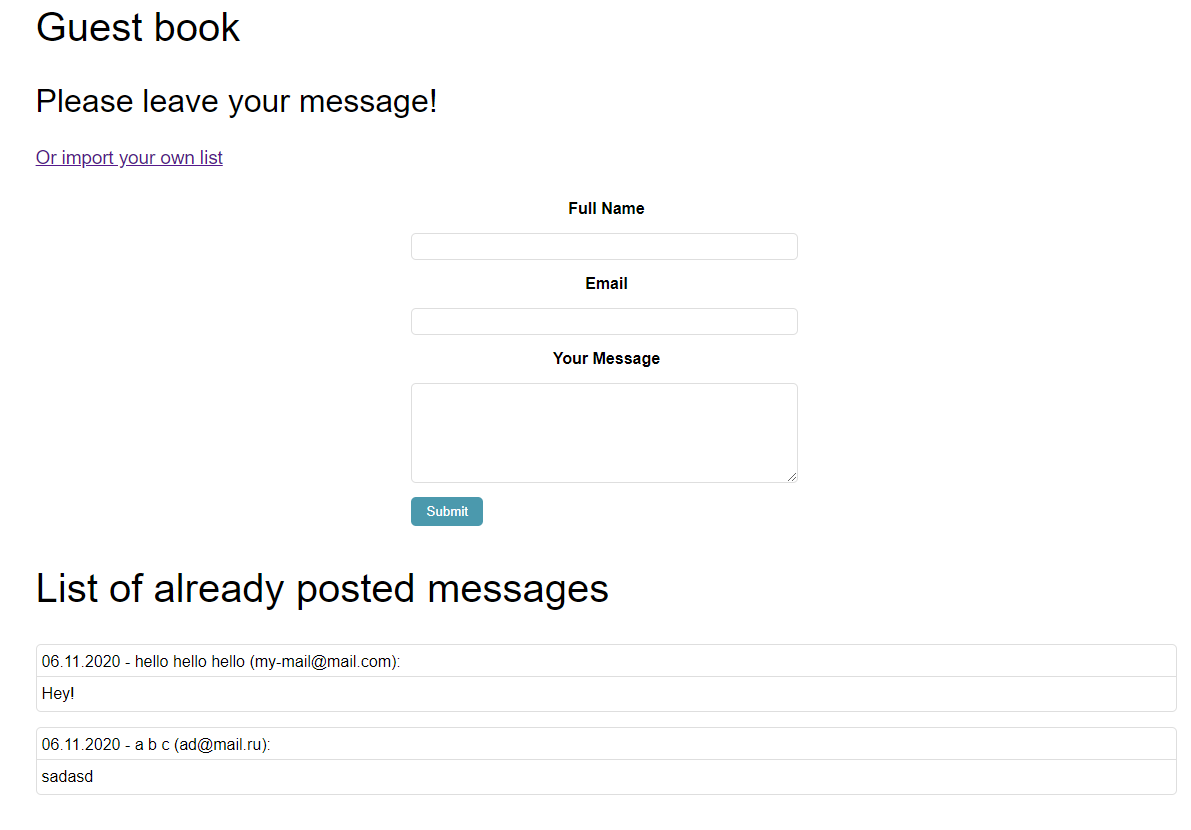
\includegraphics[width=\linewidth]{guest-book}
    \caption{Реализация гостевой книги}
    \label{fig:guest-book}
\end{figure}

\subsection{Сохранение ответов в базе данных}
Изменения в контроллере:
\begin{lstlisting}
class TestController {
    private $pageSize = 10;

    public function __construct(IContainer $container) { }

    public function index() {
        $viewModel = new ValidationViewModel(true, array());
        ViewRenderer::render("Views/Test/Index.php", "Test", $viewModel);
    }

    public function answers() {
        $page = isset($_GET['page'])
            ? $_GET['page']
            : 1;

        $offset = PaginationHelper::getOffset($page, $this->pageSize);
        $answers = Answer::findByPage($offset, $this->pageSize);

        $totalPages = PaginationHelper::getTotalPages(Answer::getCount(), $this->pageSize);
        $paginationViewModel = new PaginationViewModel($page, $totalPages, "/Test/Answers");
        $viewModel = new AnswersViewModel($answers, $paginationViewModel);

        ViewRenderer::render("Views/Test/Answers.php", "Answers", $viewModel);
    }

    public function testPost() {
        $validator = new TestRequestValidator($_POST);
        $validationResult = $validator->validate();

        if ($validationResult->isValid) {
            $answer = new Answer();
            $answer->createdAt = date("Y-m-d H:i:s");
            $answer->studentFullName = $_POST["Name"];
            $answer->email = $_POST["Email"];
            $answer->question1Answer = $_POST["Question1"];
            $answer->question2Answer = $_POST["Question2"];
            $answer->fullTextAnswer = $_POST["Question3"];
            $answer->save();

            $testVerification = new TestRequestVerification($_POST);
            $viewModel = new SuccessfulTestViewModel($testVerification->verify());
            ViewRenderer::render("Views/Test/Success.php", "Test", $viewModel);
            return;
        }

        $viewModel = new ValidationViewModel($validationResult->isValid, $validationResult->errors);
        ViewRenderer::render("Views/Test/Index.php", "Test", $viewModel);
    }
}
\end{lstlisting}

Постраничный вывод данных:
\begin{lstlisting}
private static function renderLinkToCurrentPage(PaginationViewModel $model) {
    static::renderLinkToPage($model->currentPage, $model->baseUrl, false, true);
}

private static function renderLinkToPreviousPage(PaginationViewModel $model) {
    static::renderLinkToPage($model->currentPage - 1,
                                $model->baseUrl,
                                $model->currentPage != 1,
                                true,
                                "Previous");
}

private static function renderLinkToNextPage(PaginationViewModel $model) {
    static::renderLinkToPage($model->currentPage + 1,
                                $model->baseUrl,
                                $model->currentPage < $model->totalPages,
                                true,
                                "Next");
}

public static function renderPagination(PaginationViewModel $model) {
    static::renderLinkToPreviousPage($model);
    static::renderLinkToPage($model->currentPage - 2,
                                $model->baseUrl,
                                $model->currentPage >= 3,
                                $model->currentPage >= 3);
    static::renderLinkToPage($model->currentPage - 1,
                                $model->baseUrl,
                                $model->currentPage >= 2,
                                $model->currentPage >= 2);
    static::renderLinkToCurrentPage($model);
    static::renderLinkToPage($model->currentPage + 1,
                                $model->baseUrl,
                                $model->currentPage + 1 <= $model->totalPages,
                                $model->currentPage + 1 <= $model->totalPages);
    static::renderLinkToPage($model->currentPage + 2,
                                $model->baseUrl,
                                $model->currentPage + 2 <= $model->totalPages,
                                $model->currentPage + 2 <= $model->totalPages);
    static::renderLinkToNextPage($model);
}
\end{lstlisting}

Результат представлен на рисунке \ref{fig:answers}.
\begin{figure}[H]
    \centering
    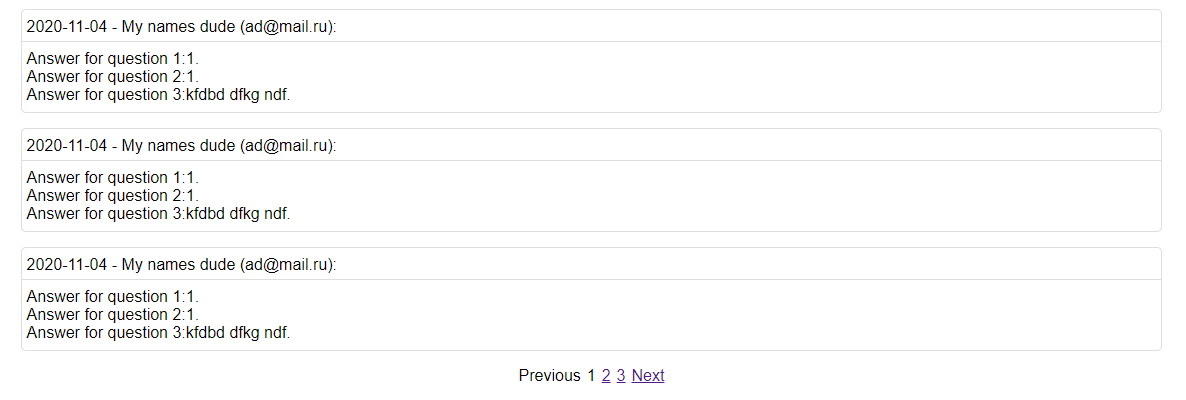
\includegraphics[width=\linewidth]{answers}
    \caption{Реализация сохранения ответов в БД}
    \label{fig:answers}
\end{figure}

\subsection{Реализация блога}
Создание контроллера:
\begin{lstlisting}
class BlogController {
    private $pageSize = 10;

    public function __construct(IContainer $container) { }

    public function index() {
        $page = isset($_GET['page'])
            ? $_GET['page']
            : 1;

        $offset = PaginationHelper::getOffset($page, $this->pageSize);
        $answers = BlogEntry::findByPage($offset, $this->pageSize);

        $totalPages = PaginationHelper::getTotalPages(BlogEntry::getCount(), $this->pageSize);
        $paginationViewModel = new PaginationViewModel($page, $totalPages, "/Blog/Index");
        $viewModel = new BlogEntriesViewModel($answers, $paginationViewModel);

        ViewRenderer::render("Views/Blog/Index.php", "Blog", $viewModel);
    }

    public function post() {
        $viewModel = new ValidationViewModel(true, array());
        ViewRenderer::render("Views/Blog/Post.php", "Post", $viewModel);
    }

    public function uploadPost() {
        $validator = new BlogRequestValidator($_POST, $_FILES);
        $validationResult = $validator->validate();

        if ($validationResult->isValid) {
            $picturePath = $_FILES["Picture"]["tmp_name"];
            $pictureName = $_FILES["Picture"]["name"];
            $picture = file_get_contents($picturePath);
            file_put_contents($_SERVER["DOCUMENT_ROOT"] . "/client-side/images/" . $pictureName, $picture);

            $blogEntry = new BlogEntry();
            $blogEntry->createdAt = date("Y-m-d H:i:s");
            $blogEntry->name = $_POST["Name"];
            $blogEntry->message = $_POST["Message"];
            $blogEntry->photoName = $pictureName;
            $blogEntry->subject = $_POST["Subject"];
            $blogEntry->save();

            $this->index();
            return;
        }

        $viewModel = new ValidationViewModel($validationResult->isValid, $validationResult->errors);
        ViewRenderer::render("Views/Blog/Post.php", "Post", $viewModel);
    }
}
\end{lstlisting}

Результат представлен на рисунке \ref{fig:blog}.
\begin{figure}[H]
    \centering
    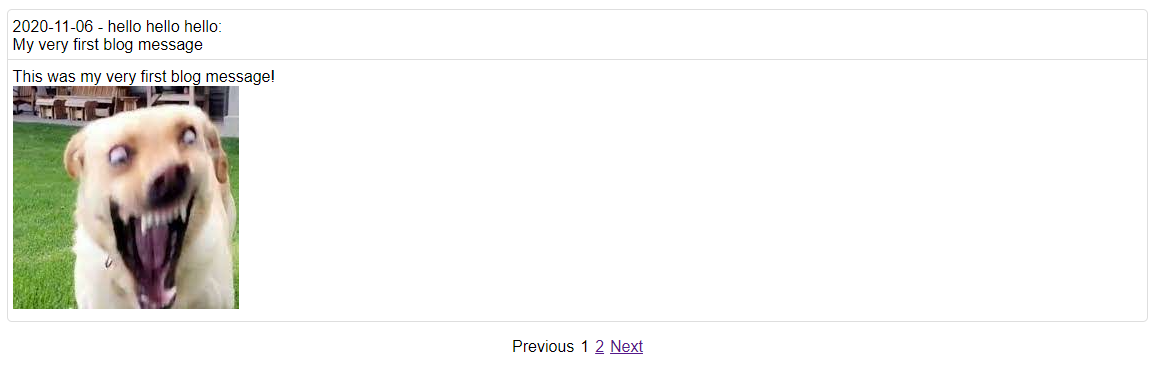
\includegraphics[width=\linewidth]{blog}
    \caption{Реализация блога}
    \label{fig:blog}
\end{figure}

Форма для добавления записей в блог представлена на рисунке \ref{fig:blog-form}.
\begin{figure}[H]
    \centering
    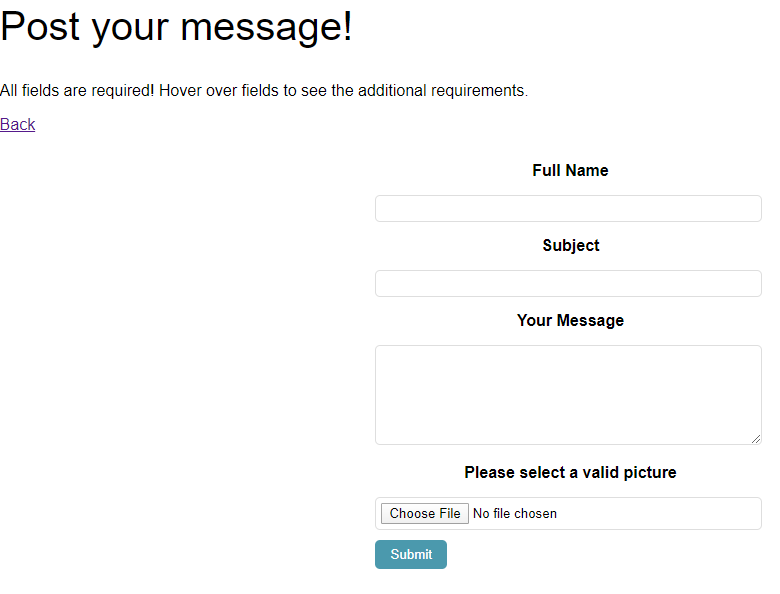
\includegraphics[width=\linewidth]{blog-form}
    \caption{Форма для добавления записей в блог}
    \label{fig:blog-form}
\end{figure}

\section*{Выводы}
В ходе лабораторной работы была изучена работа с файлами и базой данных в PHP.
Для взаимодействия с базой данных используется интерфейс PDO. Соединение с PDO
было энкапсулировано в объект ActiveRecord, который реализует все методы для
работы с таблицами базы данных.

\end{document}